\chapter{Programmazione aggregata}

La crescita esponenziale di dispositivi informatici di varia natura inseriti in contesti quotidiani ha avuto un impatto globale notevole.
Questo insieme di entità connesse (\Cref{fig:iot}) ha dato luogo a ciò che viene definito \emph{Internet of Things} (\emph{IoT}).

\begin{figure}
  \centering
  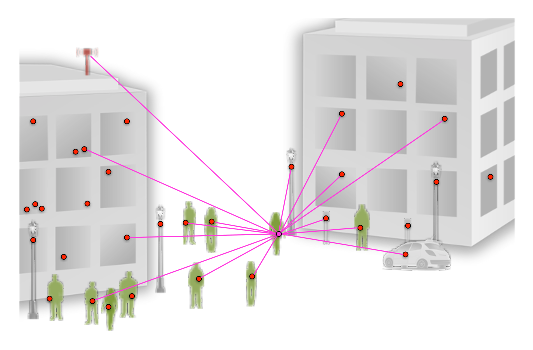
\includegraphics[width=0.8\textwidth]{res/fig/iot.eps}%
  \caption{Possibile scenario di rete in contesto urbano~\cite{7274429}}%
  \label{fig:iot}
\end{figure}

L'approccio iniziale per la realizzazione di sistemi in questo contesto è stato incentrato sui classici paradigmi ``\emph{single device view point}'',
i quali vedono al centro dell'attenzione il singolo dispositivo e le interazioni che questo ha con gli altri e con l'ambiente.
Tale approccio si è ben presto rivelato inadeguato % TODO: perché?
